
% 关于
    \section {资产概述}

.
    \begin{center}
        
\includegraphics[scale=0.2] {gold.jpg}
    \end{center}

    会计学上的资产(Asset),指一企业透过交易或非交易事项所获得之经济资源,能以货币衡量,并预期未来能提供效益者。

\subsection {资产的属性}

    依据资产的一般定义,它具有下述特性:
    \begin{itemize}
        \item  该事物存在未来的经济价值。“未来的经济价值”是指,特定企业(或组织)若拥有该事物(资产),则可以利用其来产生(增加)企业未来的现金流入,或利用其替代(减少)企业未来发生的现金流出。
        \item  该事物产权被特定企业控制。
        \item  若某事物属于资产(存在未来的经济价值),但非某企业可控制,则某企业无法利用其经济价值,故该事物对于某企业不属于资产。
        \item  若该事物属于公共财产,虽然该事物对特定企业可能存在未来的经济价值,但公共财产非被特定企业所控制,故公共财产皆不为特定企业的资产。
    \end{itemize}

    资产是财务会计中争议最大的概念之一。历来的会计学家都试图对资产给出满意的界定,但到目前为止,一个权威的、被学术界和实务界所共同认可的定义,尚未出现。

    资产的经济属性即能够为企业提供未来经济利益,这也是资产的本质所在。也就是说,不管是有形的还是无形的,要成为资产,必须具备能产生经济利益的能力,这是资产的第一要义。

    资产的法律属性即必须是为企业所控制,也就是说,资产所产生的经济利益能可靠地流入本企业,为本企业提供服务能力,而不论企业是否对它拥有所有权,这是资产的第二要义。  

\subsection {资产的分类}

    财务会计中的资产是指预计有助于生产未来现金流入或减少未来现金流出的经济资源,一般分为:

    \begin{itemize}
        \item  依据是否有具体形体分类
            \begin{itemize}
                \item  有形资产
                \item  无形资产
            \end{itemize}

        \item  依据耐用期限的长短分类
            \begin{itemize}
                \item  长期使用资产(固定资产)
                \item  流动资产
            \end{itemize}

        \item  依据资产所有权分类
            \begin{itemize}
                \item  贷方权益(负债)
                \item  业主权益
            \end{itemize}
    \end{itemize}

\subsection {资产定义的几种观点}

    未消逝成本观:未消逝成本观是对资产性质的早期描述。美国著名会计学家佩顿和利特尔顿在《公司会计准则导论》(an introduction to corporate standard)(1940)中明确提出了未消逝成本观。他们认为:“……成本可以分为两部分,其中已经消耗的成本为费用,未耗用的成本为资产……”也就是说,他们认为资产是营业或生产要素获得以后尚未达到营业成本和费用阶段的那部分余额,是成本中未消逝的那部分余额。显然,这种观点同历史成本会计模式是密不可分的。它着重从会计计量的角度来定义资产,强调了资产取得与生产耗费之间的联系。

    借方余额观:资产定义的借方余额观是由美国会计师协会(美国执业会计师协会的前身)所属的会计名词委员会在其颁布的第1号《会计名词》(1953)中提出来的。该公告认为:“资产是由借方余额所体现的某种东西。这一借方余额是按照公认会计原则或规则从结平的各账户中结转过来的,前提是这一借方余额不是负值。作为资产,它代表的或者是一种财产权利,或者是所取得的价值,有的则是为取得财产权利或为将来取得财产而发生的费用支出”。这一认识的基本特征是将资产视为借方余额的体现物。据此,不仅借方余额所体现的应收账款、存货、设备、厂房等要确认为资产,而且由借方余额所体现的递延费用等项目也可以确认为资产。显然,这种观点只是从会计结账技术的角度来理解资产,很难说是在描述资产的性质。

    经济资源观:经济资源观是关于资产定义的颇具影响的一种观点。1957年,美国会计学会发表的《公司财务报表所依恃的会计和报表准则》中明确指出:“资产是一个特定会计主体从事经营所需的经济资源,是可以用于或有益于未来经营的服务潜能总量”。对资产的这一认识,第一次明确地将资产与经济资源相联系,虽然它并未正面提到无形资产的内容,但这一定义至少可能将无形资产包纳其中。另外,它也明确了资产与特定会计主体之间的关系,即特定会计主体能够借助资产业从事未来经营。1970年,美国会计准则委员会在其发布的第4号公告中提出了一个资产定义:“资产是按照公认会计原则确认和计量的企业经济资源,资产也包括某些虽不是资源但按照公认会计原则确认和计量的递延费用”。这一定义虽然明确指出资产的实质是经济资源,接受了“经济资源”这一新认识,但它却认为,经济资源应否视为资产,取决于公认会计原则的确认和计量标准,这就把资产的实质与资产的确认和计量之间的主从关系颠倒了。

    未来经济利益观:目前比较流行的资产定义体现了未来经济利益观的观点。1962年,穆尼茨(moonitaz)与斯普劳斯(r.t.sprouse)在《会计研究论丛》第3号——《企业普遍适用的会计准则》这一文献中明确提出:“资产是预期的未来经济利益,这种经济利益已经由企业通过现在或过去的交易获得。”现在的美国财务会计准则委员会(fasb)在《财务会计概念公告》第6号(sfac no.6)中提出:“资产是可能的未来经济利益,它是特定个体从已经发生的交易或事项中所取得或加以控制的。”

    未来经济利益观认为,资产的本质在于它蕴藏着未来的经济利益。因此,对资产的确认或判断不能看它的取得是否支付了代价,而要看它是否蕴藏着未来的经济利益。在现实中,虽然成本是资产取得的重要证据之一,而且成本还是资产计量的重要属性,但是,成本的发生并不一定导致未来的经济利益,而未来经济利益的增加也并不必然会发生成本,例如,业主投资、接受捐赠等。所以,未消逝成本观将未耗用的成本看成是资产,视资产为成本的组成部分,是不切实际的。而经济资源观强调资产的经济资源属性,把一些不是经济资源但有助于实现未来经济利益的或减少未来经济损失的项目如某些备抵项目排斥除在资产之外。未来经济利益观则将这些项目合乎情理地包括在资产之中。因此,我们说未来经济利益相对于其他观点来说更加全面、合理。


\section{销售机会管理}
    % 发现
        \subsection {销售机会发现:寻求已存在的销售机会}

    企业要从被人们忽略和丢弃的未被满足的市场需求中寻找销售机会,其途径有:

    \subsubsection {从供需缺口中寻找销售机会}

    某类产品在市场上供不应求时,就表明了可供产品在数量、品种方面的短缺,反映了消费者的需求尚未得到满足,这种供需缺口对于企业来说就是一种市场机会。寻求供需缺口可采用以下方法:

    \begin{enumerate}
        \item 需求差额法。即从市场需求总量与供应总量的差额来识别市场机会。可用公式表示:

        需求差额=市场需求量-产品供应量

        产品供应量=国内产量+进口产量+库存量

        \item 结构差异法。即从市场供应的产品结构与市场需求结构的差异找寻市场机会。产品的结构包括品种、规格、款式、花色等。有时供需总量平衡,但供需结构不平衡,仍然会留下需求空缺,分析供需结构差异,企业便可从中发现市场销售机会。

        \item 层次填补法。即从需求层次方面来寻求市场机会。市场需求层次可分为高、中、低三档。马斯诺又把需求层次分为五个等级,可以通过分析各层次需求满足的情况,找出未被满足的“空档”,并生产相应产品予以填补。
    \end{enumerate}

    \subsubsection {从市场细分中寻求销售机会}

    从细分市场中寻找销售机会的主要方法有:
    \begin{enumerate}
        \item 深度细分。即把某项细分标准的细分程度加深拉长。如按服装型号可分为小、中、大号。但如果采用延伸法把细分度拉长,则可分为:特小号、小号、中号、大号、特大号和特型号等,也可将细分度加深,如特型号中分宽长型、宽短型、窄短型等。深度细分,照顾了消费者复杂的需求差异,通过这次细分,可以发现未被满足的市场。

        \item 交叉细分。即采用两上标准细分。例如家俱可以用收入、年龄两个标准细分市场,可以把市场分成若干个次市场。

        \item 立体细分法。即采用三个细分法。如按收入、年龄、人口三个标准细分,可以把市场分成(3×3×3)27个次市场,这27个市场各不相干。

        \item 多维细分法。即采用多种标准对市场进行细分,如按文化程度、购买动机、生活方式、年龄、职业、收入等细分市场,可以细分出更多的市场,从中发现被他人忽略的市场机会。
    \end{enumerate}

    \subsubsection {从产品缺陷中寻求销售机会}

    产品缺陷往往影响消费者的购买兴趣及两次购买的可能,不断弥补产品的缺陷则可能给企业带来新的生机。例如:某生产照相机企业,最初投放市场照相机机型复杂、笨重、不易操作,针对上述缺陷,研制推出一种快速自动照相机、弥补了原照相机的不足,产品一上市大受欢迎。以后,他们又在消费者调查中了解到该相机闪光灯需用电池带动,经常更换电池给消费者带来麻烦,而且电池留在机内时间长了会变质漏水,损坏照机。为克服这些缺点,研制人员研制出一种更趋完美的能够弥补上述缺陷的超小型、匣式、不用电池的新型照相机,新式相机很快行销市场。

    \subsubsection {从竞争对手的弱点中寻求销售机会}

    研究竞争对手,从中找出竞争对手产品的弱点及销售的薄弱环节,也是寻找机会的有效方法之一。如:某家大电器公司,以“取竞争者之长,补竞争者之短“的方式,参与市场竞争。在竞争对手成功地开发出自动洗碗机之后,就把这种洗碗机带回实验室,从产品功率、性能、零件数量和种类及成本构成等逐一进行评估,该公司将机器拆散,对每个零件加以研究,以发现弱点加以改进。这样,这家公司很快地开发出一种性能更好,价格更低的全自动洗碗机,从而取代了竞争对手。

\subsection {销售机会的捕捉诀窍}

    捕捉销售机会,对销售人员各方面的能力有较高的要求,它要求销售人员能够及时收集并分析研究影响推销环境变化的因素的信息和资料,从中发现销售机会出现的可能性和具体内容;要求销售人员能看准时机,以恰到好处地捕捉销售机会;要求销售人员能发挥主观能动性和创造性,善于打破常规,创造出独具特色的销售机会;要求销售人员注意把握因地制宜的原则,研究销售机会的空间适应性。

    捕捉销售机会虽然并不容易,但也并非无窍门可寻。以下介绍几种捕捉销售机会的诀窍:

    \begin{enumerate}

    \item 谨思慎行

    推销工作的每一个步骤对销售人员来说都极为重要。销售人员处理得当,有可能促成推销机会的出现和形成;但若销售人员急于求成,鲁莽行事,则有可能亲手毁灭销售机会出现的可能性。

    因此,销售人员在推销的每一环节都应保持冷静,随时掌握局势的变化,利用自己的常识和经验,充分分析思考,然后再谨慎行动。切勿信口开河,鲁莽行事,使顾客产生不信任感,或由于压力过高而丧失购买信心,从而失去有利的销售机会。

    \item 察言观色

    在推销过程中,销售机会往往都是潜生的,具有相当的隐藏性,而不会明显地显现出来,但也并非是完全无迹可寻的。顾客的购买倾向和成交意愿往往会从顾客的表情、语言、行为等方面显现出来,因而销售人员应善于观察和分辨,依据自己的推销经验及时捕捉推销机会。

    \item 多听少讲

    销售人员一接近顾客,马上口若悬河,恨不得将推销品全部优点一股脑儿告诉顾客,这是推销工作的一大忌。销售人员应虚心听取顾客的意见和要求,而不要只顾自己讲话(应在必要时予以回答)。这样不但让顾客感到受到尊重,从而有利于创造良好的推销氛围,并且可以从顾客的言谈中获得推销的线索和答案,从而控制推销机会。

    \item 循序渐进

    推销交易有简有繁,复杂的交易往往需要多个回合才可能完成。因此,销售人员应有足够的耐心和恒心。循序渐进,按部就班,配合推销活动的每个阶段适时地把握机会,调整推销工作的方式和内容。不要急于求成而破坏了有利的销售机会。

    \item 耐心等待

    耐心是销售人员必须具备的重要品质。急功近利,行事冲动极易导致推销失败。这是因为,顾客在做出买不买,买多少,何时买等购买决策时,都不是一时冲动可以决定的。他需要权衡各种客观因素,如产品特征,购买能力等,同时还要受到主观因素的影响,如心情好坏等。因此,购买决策过程是一个极其复杂的过程,并不是一蹴而就的。销售人员应设身处地地为顾客着想,体会顾客的难处,耐心地等待时机。

    另外,销售人员和顾客双方有各自不同的习惯和想法,考虑问题和行事的方法和程序也都各不相同。在推销过程中,销售人员不能将自己办事的程序强加于顾客,而应注意顾客的思路,调整自己以与之相配合。因此,有足够的耐心,是选择竞争时机的关键。但销售人员也不应一味地消极等待,在关键时刻要发挥推波逐澜的作用,以免贻误时机。

    \item 坐山观虎斗

    当别人出现失误时,可能你的好机会就来了。在推销活动当中,推销的参与者之间往往存在着种种矛盾,利用这些矛盾经常能为自己创造出难得的机会。

    首先,要利用顾客和竞争对方之间的矛盾。在顾客向你抱怨竞争对手时,你应该乘机而入,向顾客推销自己的商品,有可能会获得成功。这虽然是落井下石的作法,但切不可给顾客以落井下石的感觉,以免顾客产生反感。因为你作为竞争对手的身份是比较敏感的,一定要把握分寸,不要不择手段,把对方贬低得一无是处,并注意一定要以事实为根据来说话,才会更有说服力,从而赢得顾客的信任和好感。

    其次,要利用竞争对手之间的矛盾。竞争对手之间,出于利益的争夺,往往存在着种种矛盾。有时,双方会你争我夺,在顾客面前互相贬损,甚至有时会不惜亏本,一决雌雄,最终很可能弄得两败俱伤。在这种情况下,你应冷静观察,在双方争夺激烈时按兵不动,当双方筋疲力尽之际,再伺机出击,展开推销攻势,争取顾客。

    \item 伺机而动

    一些特殊日子和事件往往是推销商品的大好时机,如我国传统节日春节、元旦、国庆节等重大节日,各种体育盛会,纪念活动等都有可能成为推销商品的大好机会。有经验的销售人员往往能事先就做好充足准备,拟定销售计划,做好万全之策,把握并利用这些机会,极力宣传商品,刺激顾客的购买欲望,促进商品销售。

    \item 环境烘托

    销售人员还可为顾客创造良好的购物环境,并根据商品的特点,设计柜台摆放,商店装潢、灯光设计、商品包装、背景音乐、环境卫生等环境条件,来衬托并突出商品,增强商品竞争能力,激发顾客的购买欲望,从而促进商品销售。

    \item 节奏缓急

    销售人员把握推销节奏的能力极为重要。在该给予顾客思考权衡时就应放缓节奏,给顾客喘息的机会。而在销售人员发现有迹象显示出顾客的购买意图时,则应抓住时机,一鼓作气,劝说顾客,达成交易。

    \end{enumerate}

\subsection {创造新的销售机会}
    创造销售机会在于能对销售环境变化做出敏捷的反应,善于在许多寻常事物中迸发灵感,巧于利用技术优势开发出新产品。

    \subsubsection {从市场发展趋势中创造销售机会}

    市场发展趋势包含两方面内容:一是指某类产品市场(包括销售、消费、需求)增长比率;二是指市场客观环境的变化动向。

    1. 增长比率法。市场增长比率的正变化,表明了未来市场需求的增长,企业应以超前的眼光,创造销售机会。例如据科威特有关机构预计今后5年科威特电讯设备需求量平均增长率为22~25\%,电讯辅助设备需求量将平均增长11~15\%,空调冷藏设备需求量平均增长18~23\%,而上述三种产品的60\%需要进口。这是企业电子产品进入科威特市场的良机。

    2. 环境变化法。即从市场宏观环境变化中创造机会。环境往往使机会与挑战并存,经营者既要以敏锐的眼光从变化动向中预测未来,把握销售机会,还要以非凡的创造力,善于把挑战转化为机会。例如:在我国大中城市中,人口出现老龄化趋热,这意味着老年人市场逐步扩大,企业可把握此动向,深入细分老年人市场,开发出能最大程度地满足他们要求的各种产品。

    \subsubsection {从社会时代潮流中创造销售机会}

    社会发展的各个时代都会形成流行的涡心,例如当今时代的潮流是回归大自然。在这种社会大潮的冲击下,许多企业顺应潮流,把握机遇,推出了“自然产品”,如用植物原料制造出的药品、化妆品、饮料;开发出“绿色产品”(即减少环境污染、保护生态环境、节约使用自然资源的产品)。由于这些产品迎合了当代人们的心态,从而激发了人们新的需求。

    \subsubsection {用科学技术创造销售机会}

    现代科学技术的发展趋势,表现出三大特征:

    1. 新材料的应用。近年来世界新材料的开发主要集中在高功能聚合物、精密陶瓷、复合材料和高级合金上。目前这类新材料市场规模达2000亿美元,预测到2000年,上述4种材料成交额可超过100亿美元,研制并抢先运用这种新材料,推出新产品,能创造新的市场机会。

    2. 新能源的利用。即用新的能源取代旧的能源。如国际鉴于石油资源的短缺,正在研制新的能源汽车等,如电动汽车、甲醇汽车、天然气汽车、太阳能汽车和氢气汽车等。

    3. 新技术的应用。21世纪将是电子化的时代,将电子技术广泛地应用到生产领域可以创造新的市场机会。总之,随时关注世界科学技术发展动态,及时地将这些技术引入生产领域,将给企业带来无限生机。

    \subsubsection {用销售手段创造销售机会}

    通过采用创新的销售手段,创造新的销售机会。例如,日本阿托搬家中心,改变过去搬家方式,别出心裁,决意要将“烦恼的搬家”变为“愉快的旅行”由此设计出一种命名为“21世纪的梦”的搬家用车,这种车分为上下两层,上层前半部是豪华客厅和休息场所,娱乐设备齐全,下层是驾驶室,车的后半部为行李车厢。阿托中心还同时提供3000多项与搬家有关的服务,此车一推出,预约搬家者蜂拥而至。这是通过创新的服务来创造新的销售机会。此时还可通过预报商品流行,来引发消费者的需求,如预报服装家俱流行款式、流行色;还可以利用广告宣传、新闻报道等创造销售机会。

    企业一旦识别和寻求到恰当的销售机会,必将为企业的经营与发展带来勃勃生机。

\subsection {销售机会的评估}

\begin{enumerate}
    \item 分析销售机会的性质
        \begin{enumerate}
            \item 明确成功利用某一机会的必要条件;
            \item 以利用这一机会的基本要求为参照,分析本企业从事相关业务的能力,确认利用这一机会的优势与不足,弥补差距的可能性;
            \item 同样分析每一个最有可能的竞争者;
            \item 比较本企业与竞争者,各自在成功利用这一机会条件方面的优劣,确认本企业对这一机会是否拥有相对竞争,差距大小。
        \end{enumerate}

    \item 分析销售机会的质量

        \begin{enumerate}
            \item 分析这一机会所显示的,仅仅是人们的需要和欲望,还是已经形成市场。暂时条件不允许,或人们不打算经由市场满足的需要,至多只是一个潜在的市场。
            \item 分析这一市场是否拥有起码的规模,即是否有了足够数量的顾客;
            \item 确认本企业进入这一已有足够数量顾客的市场,是否具备必需的销售能力。
        \end{enumerate}
\end{enumerate}

    % 管理
        \subsection {销售机会管理方法}

    销售机会管理有很多不同的名称,常用的名称有商机管理和销售漏斗管理,适用于大型复杂订单的销售,常用于直接销售和专卖店销售两种模式。

    96年,IBM在中国开始推行销售机会管理,现在已经形成了一套完整的体系,并且依赖这个体系来驱动销售目标的实现。

    每周一,销售人员将销售报表交给直接的主管,并在部门会议中逐一分析重要的销售机会,确定行动计划;周二,销售主管汇总自己的所有销售机会,与二线主管进行汇报,并讨论确定的销售计划;周三,二线主管与中国区的主管汇报和讨论销售机会和销售行动;周四,中国区的主管将汇总的报表交给亚太区的主管,取得他的认可;周五,全球的报表就到了全球总裁的桌面。IBM就是这样由下到上进行销售机会的管理。

    销售机会管理的本质是通用的公司用于管理销售机会的工具和方法。虽然不同的公司的称呼不一样,但跨国公司对于大型和复杂订单几乎都采用类似的工具。这种方法提供了销售团队关于进行沟通的语言,例如各个销售阶段的定义,并且提供了衡量销售机会和关键的过程性的指标。

    销售机会管理也体现了大型订单销售的精华,销售人员应该能够识别采购阶段,针对不同客户采取不同的销售策略。

    销售机会管理包括表格或者系统中的部分,也应该包括系统外的定期的销售会议,进行讨论、行动计划、反馈和总结。

\subsection {销售机会的分级}

    张学生以前是一家大公司的销售代表,他的太太就职于另外一家大型公司,他们在五年前买了一辆富康轿车。由于工作繁忙,没有时间学车,这部车一直由太太驾驶。

    一年前,他离开公司自己创业,开了一家印刷公司。由于需要经常在公司外与客户应酬,因此考了驾驶执照,开始开车。客户搭车的时候,富康安明显感觉到富康不能体现公司的形象,因为它与一家成功公司的总经理很不协调。因此希望换一部车。

    他的家里只有一个孩子,每个月的纯收入大约在两万元左右,因此他们商量后,决定购买一辆既能家用又能公司用的国产的中高档轿车。

    周末,他与太太常常去各个品牌的专卖店,已经看过雅阁、君威、奥迪和宝马。陆续排除了雅阁和君威,决定在奥迪和宝马中选择一辆。

    半年前,两人多次去看了宝马和奥迪的专卖店,张先生很喜欢奥迪A4,太太喜欢宝马325。由于担心汽车降价,因此两人决定持币观望,再等等。

    终于,听说奥迪开始于七月份做促销,可以得到额外的折扣,因此两人去专卖店查询。两人获知,除了折扣外,还可以额外得到大约一万元的折扣。

    两人去其它奥迪专卖店去进行了比较,包括价格,折扣和服务,最终选择了距离自己家和公司较近的专卖店。在专卖店的销售人员安排下,进行了试驾。

    之后,与销售代表进行谈判,确认了价格和赠送的配置。本来,两人还想再等等,但听说奥迪A4原装的CKD的产品只剩两台,以后就是SKD组装的,因此迅速将这台奥迪A4在国庆前买回家。

    没想到,十一刚过,就得到了奥迪降价的消息,这让他们很不满意,因此与奥迪专卖店交涉。在没有结果的情况下,他们非常不满意。最近,他的一位朋友也希望买奥迪,富康安坚决推荐他去另外一家专卖店购买。

    像案例中的客户一样,一家汽车销售公司有很多这样的销售机会,所有的订单都是从这些销售机会中产生的,如何管理这些销售机会呢?首先,我们要将案例中机会分成几个阶段。

\subsection {销售机会的管理指标}

    销售人员要识别客户的采购阶段,因为在不同阶段客户关心不同要点。对于向大型机构的采购,不同的客户在不同采购阶段起到主要的作用。

    \begin{center}
        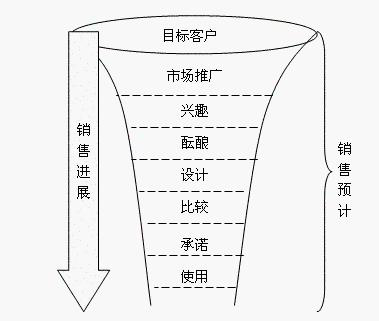
\includegraphics[scale=.6] {loudou1.png}
    \end{center}

    识别销售机会的阶段后就可以对销售机会进行管理了。我们可以将销售想象成一个漏斗,一些销售机会漏掉了,有一些销售机会经过采购流程的各个阶段转变成为订单。销售漏斗中有足够的销售机会并且不断地向下流动,转变成订单,直到达成销售目标。衡量销售机会是否足够的指标就是销售预计,衡量销售机会是否向下流动的指标就是销售进展。这两个量化的指标就是销售漏斗管理的核心的过程性指标。

    \begin{enumerate}
        \item 销售预计:

        销售团队或者成员中,处于各个采购阶段的销售机会的金额乘以这个阶段赢率的总和。销售机会可以用下面的计算公式表示:

        销售预计=∑(销售机会额X阶段赢率)

        每个销售人员必须有足够多的机会才可以完成任务,如果销售预计小于剩余的销售任务,那么销售人员就需要继续寻找销售机会。

        \item 销售进展:

        销售进展表示销售团队或者销售人员的销售机会转变成销售订单的速度。通常上市公司每个季度公布自己的财务数据,而销售管理又是以周进行。销售进展是根据每周的销售数字与季度的销售任务,计算后得到的。

        销售进展的计算方法是:本周销售预计加上本周累计销售额减去上周销售预计和上周累计销售额除以本季度的销售任务。由于一个季度有十三个周,因此销售人员每周的进展应该达到7.8%。

        \item 漏斗外销售额:

        对于为了使得销售漏斗管理简单易行,避免大量的录入工作,很多小型订单必须排除在销售漏斗以外。通常是以订单的金额为界限,低于一定金额的订单就不纳入销售漏斗管理。由于这个这个指标,销售预计和销售进展的计算公式要进行适当的修改。
    \end{enumerate}

    通过上述三个过程性指标就可以很好的管理销售多个机会,对每个目标客户分析需要更加深入的分析方法。


\section{销售跟进}
    % 客户跟进
        \subsection {目标客户跟进}

    我们都知道,生意往往不是一次就能谈成的,需要反复多次的商讨和沟通才能够达到双方都比较满意的效果,而最终签单。这中间的过程,就需要我们的销售人员不断地跟进,使得谈判不断地深入,从而达到我们预计的目的。

    客户的跟进是需要技巧的。首先我们要明白客户跟进的目的是什么:

     \begin{enumerate}
        \item 动态的了解客户方的需求变化,并依此调整自己的销售策略

        \item 不断重申自身媒体价值和能够给客户方带来的收益

        \item 增进与客户方负责人的感情,减少交易障碍
     \end{enumerate}

    在我们理解了客户跟进主要目的后,接下来的问题是怎样进行跟进:

     \begin{enumerate}
        \item 拜访跟进:

        最推荐的客户跟进方式。当面交流可以更直观的了解客户公司的动态和需求变化,同时可以增进彼此的感情和信任度。一般处于售前阶段的跟进以每周一次为宜,但如遇特殊时期(例如:直接竞争对手正在于我们抢份额;客户方制定年度计划期间),可以考虑2-3天进行一次拜访跟进。

        \item 电话跟进:

        比较节省时间的跟进方式。在电话跟进时切忌流于“程式化”,一定要在同电话前做好准备:确定通话目的;要通过电话向对方了解什么;准备通过电话告诉对方哪些有益的或对方感兴趣的信息;设计好通话的开场白和“问题漏斗”等等。

        \item 资料跟进:

        通过向客户方发送相关资料,达到增加与客户合理接触机会的目的;达到增加销售机会的目的;达到与对方增进感情、消除隔阂的目的;并最终达到刺激客户购买本媒体广告的目的。这些资料包括:新的招商计划方案;价格变动信息;已发布过的同业网络广告检测记录;已执行过的目标客户竞争对手的专项活动总结报告;最近计划进行的公关或促销活动或论坛活动方案等等。

        \item 服务跟进:

        邀请客户相关负责人观摩我们组织的各项活动,有限度的参加我们组织的公关或促销活动,让客户感受我们的平台价值和服务价值,从而刺激其购买欲,最终促成成交。

        \item 负责人公关:

        了解客户方“关键人物”的脾气秉性、兴趣爱好、生活习惯、性格弱点等等,投其所好,消除隔阂和对立情绪,与之建立良好的、可以互相信任的个人关系。
     \end{enumerate}

    客户跟进的最终目的是:通过不断的、高频率的信息和服务“轰炸”,与目标客户达成“互信”,并使目标客户越来越清楚的认识到搜房平台与专业服务的价值,刺激目标客户与本媒体合作的欲望,从而最终达到“销售签约、顺利收款”的目的。因此,以上所列举的各种跟进方式可以根据目标客户的不同特点,组合运用。

        \subsection {客户跟进技巧与实例分析}

    现在无论是做网络营销还是电话营销,客户跟进都很重要,因为客户有时候是需要我们保持长期联系的,一旦你不联系客户,客户有可能就改变主意了或者是觉得你的服务有问题。因此,我们就来看看客户跟进的技巧与话术吧。

    我们举个例子来说明,当我们在电话中与一些客户初步交流过后,客户可能会讲:“好,你给我些资料看看。”而当电话营销人员在发过电子邮件后,再打电话跟进的时候,可能会有如下场景:

    销售人员:“今天给您电话,就是想同您确定下资料是否收到。”

    客户:“收到,谢谢!”

    销售人员:“那有什么疑问的地方没有?”

    客户:“没有,谢谢!”

    销售人员:“如果是这样,那让我们保持联系,如果以后有什么需要的话,请随时与我联系!”客户:“好的,好的,一定,一定!”

    这个跟进电话是否很成功,相信经验丰富的电话销售人员会说:“不。”因为经验告诉我们:这样讲的客户80\%以上不会再主动与你联系。那如何打跟进电话才会既可以推动销售,又可以保持长期关系,又可以加强客户对我们的良好印象呢?

    首先,要在第一次电话中确定这个客户是否值得你再次打电话给他,否则,就是在浪费时间。

    电话目标很重要,像刚才例子中,除了知道客户是否收到资料外,还应尽可能多的提些问题,获取更多的信息。例如:

    “那这个问题您怎么看?”

    “它对有帮助吗?”

    “帮助在什么地方?”

    “您建议我们下一步如何走?”

    “为什么呢?”等等

    跟进电话在开始白中把这次电话与上次电话的要点和结果联系起来,让客户想起上次谈话的要点,如双方都做过的承诺等,同时,陈述这次电话目的。而不是仅仅告诉客户:“我觉得应打个电话给您…”。

    典型的跟进电话:

    “陈经理,我是**公司的***,上周三电话结束时,我们约好今天打电话给您。当时,我们谈到…,今天给您电话是我们对这个问题又进行了深入研究,想同您探讨下这个结果,可能会花15分钟左右,现在打电话方便吗?”

    打跟进电话给客户时,最好能有些新的、有价值的东西给客户,让客户觉得每次与你通完电话后都有收获。关于这一点,最好能与你的同事一起进行头脑风暴,看看可以找出多少有价值的理由与客户保持联系。例如,你公司最新的产品、同客户约好回电、客户在这期间业务上发生了变化、同客户确定价格等等。

    “我们公司最近根据客户的要求,开发了一种新的成本更低的产品…”

    “最近看到您公司业务在调整,所以,想着您可能会需要我们的帮助…”

    “最近在看报纸,其中的一条新闻觉得您可能会感兴趣…”

    “我一看到我们的新产品,我第一个想到的就是您,我觉得您可能从中获得利益…”

    “我昨天看电视,听到一个主持人的声音特别像你,所以,就打电话给你…”

    打跟进电话时以下话语尽可能少讲:

    “打电话给您主要是想看看您最近好不好...”

    “是看看是不是有什么变化…”

    “很久没有联系了,觉得应当给您个电话…”

    “只想看看您是否准备好…”

    “看是不是有些什么东西是您需要的…”

    但这些话可做为已成交客户的回访话术

    跟进电话的一般流程:

    表明身份”我是XX公司的XX…”

    从某点上过渡到这个电话目的“上个星期您提到…”

    打电话目的“今天就是具体同您一起探讨那个降低成本的计划的”

    确认客户时间是否允许“可能要花10分钟时间,现在方便吗?”

    提问问题把客户引入会谈“您对我提交给您的新方案有什么建议?”

    做好计划,识别有价值客户进行跟进,根据不同类型的客户确定电话跟进的频率,最好一个客户联系软件来管理你的客户,以提高效率。

        \subsection {销售中的沟通方法}

    人们往往认为,商品市场中的销售者只是在销售商品。其实,从沟通学的角度,从更高的层次来分析,销售者销售的其实是“人”。这才是买卖成功的秘诀,也是商品销售的最高境界。因为买卖双方如果认可了对方的“为人”,才更会在欲望的基础上形成动机,采取行动,完成买卖。古今中外,莫不如此。

    销售是一项沟通的艺术,把话说到客户心里,也就有了成交的希望。良好的沟通将会贯穿于销售工作的整个过程,而沟通能力的强弱,也将在每一个环节上,对销售工作的成败产生决定性的影响。销售不懂沟通学,就犹如在茫茫的黑夜里行走,永远只能误打误撞。事实上,销售高手往往都是沟通专家。

    你看“悟”字,竖心旁,五个口,那你就经常跟人沟通嘛,用心跟五个人交流,这五个人也用心跟你交流。如果你能找到五个跟你用心沟通的朋友,那你这一辈子真的就能悟到道了。了解对方想听和不想听的、喜欢和不喜欢的,以及对方的担心、顾虑等,如此便打开了人与人之间沟通的大门。高品质的沟通,应把注意力放在结果上,而不是情绪上,沟通从心开始。沟通能力是评价一个人素质高低的重要指标,沟通对于企业的重要性更是不言而喻。

    专家研究表明,优秀经理70\%以上的时间都用在了沟通上。经理如此,销售代表也不例外。因为销售代表不但要管理客户,还要管理客户的下家,也就是要协助客户做好“助销”工作,工作的内容和难度增加了。具体来说销售代表要管理好客户的物流、资金流、信息流,还有客户的下家。这“三流”的管理是建立在和客户的良好沟通上。只有良好的沟通才能落实公司的策略、定货、促销等。对客户如此,对内部也同样,在日常工作中,销售代表要和上司沟通,争取销售政策、促销活动经费等资源;和同事沟通,来争取到物流的配合、财务的配合、培训支持的配合、行政的配合等。

    “企”字由“人”和“止”组成,企业无“人”则“止”。可见:“人”是企业的第一要素!而毛主席说:有人群的地方则一定有左中右。陶行知和学生的沟通明显属于团队沟通——在企业团队,复杂的人际关系使很多人往往不善于沟通胡一夫老师认为,人与人之间的交流和沟通是一门重要的管理艺术。

    松下幸之助有句名言:“企业管理过去是沟通,现在是沟通,未来还是沟通。”因此,管理离不开沟通,沟通已渗透于管理的各个方面。正如人体内的血液循环一样,如果没有沟通的话,企业就会趋于衰亡和倒闭。胡一夫老师认为,我们的营销团队十分需要沟通,在一个团队里,如果听不到一点异响,听不到一点反对意见,那是不正常的。水,在污泥塘里,不动不响,那是死的;在清江河里,汹涌奔腾,那是活的。有一点逆耳的话在耳边响着,警钟常鸣,不见得就是坏事。甚至可以说,是好事。

    如果说“传统”逢人只说三分话,而“现代”不过是“不管三七二十一,反正有话就要直说”。那么,传统与现代的区别,几乎局限于“成熟”与“浅薄”,根本和进步与否无关,我们怎么能够盲目地反传统、崇现代呢?反过来说,“现代”的“有话直说”若是“也要适当地配合情境来掌握分寸”,请问与“传统”有什么不同?难道“由不懂得传统道理的人,将自己认为西方有的、我们没有的翻译过来,就成为现代”吗?偏偏现代社会,充满了“知东不知西”或“知西不知东”的人,又何以沟通东西两方的文化呢?

    全世界的人,都希望有话直说。却由于各地的风土人情有所差异,因而产生不同的沟通方式,这是民族性的区别使然。中国人喜欢自由自在、不受约束,当然也乐于有话直说。但是太多“先说先死”的案例,使得我们深切体会“祸从口出”的道理;因而主张“慎言”,做到“应该有话直说的时候,当然应该有话直说;不应该有话直说的时候,当然不应该有话直说”的“中道”境界,形成中国人的沟通功夫。

        \subsection {避免丢失客户的方法}

    作为销售员我们很期待的一件事就是自己能够拥有老客户,这些客户的忠诚度影响着你的业绩。想要成为优秀的销售人员一定要瞄准自己的客户,那么就从怎么不失去客户做起吧。下面就分析一下失去客户的原因。

    \begin{enumerate}
        \item 粗鲁、漠不关心或事前不准备,例如对客户提出的需求忘记或不予理会,拜访客户前的资料准备不充分。

        \item 不清楚谁是负责人,一直告诉客户说自己要上级汇报,这样会失去在客户心目中的价值与信任感。

        \item 不知所云,浪费顾客时间,永远记住与客户沟通的机会是非常宝贵的,珍惜每一分钟与谈话的机会,提高销售效率。

        \item 夸张你产品的利益或服务,会给客户带来不信任感,信任感是销售过程的基础。

        \item 隐瞒产品的注意事项,省钱的选择或已提前登场的新品,知道产品的细节是客户的权利,永远要尊重客户的权利。

        \item 尽力从每次交易中,榨取每分钱,完全没有诚信度,好的销售是会“放长线钓大鱼的”。

        \item 频繁改变交易方式,会令客户反感,质疑你的公司品牌价值,对建立长期销售关系非常不利。

        \item 交易后,不致电给顾客,以确认一切都没有问题,99\%的努力会因为这1\%的疏忽而付诸东流。

        \item 不履行你所承诺的事情,没有任何一个客户愿意和没有诚信的销售长期合作的。

        \item 不回电或回复邮件,尤其当问题发生时,细节是每个销售过程成功与否的关键因素。
    \end{enumerate}

    % 客户关系
        \subsection { 销售如何做好客户关系管理}

    现在不少的销售人员都在为寻找自己的客户发愁,有时候不是因为找不到客户,而是有了太多的客户不知道怎么办。如何做好客户管理工作呢?   其实对于客户的管理无非也就是以下几个阶段:
      \begin{enumerate}
      \item 客户信息收集
      \item 客户划分
      \item 客户跟踪处理。
        \end{enumerate}

    这其中最关键的就应该是客户的划分和跟踪处理了。那对于客户的如何划分也就决定了怎么样跟踪处理客户信息了。

    我们首先来看客户的划分,对于手上现有一个客户信息,我们可以从以下四个角度产生四种不同的划分方式。

    第一,我们可以从客户是否已经和我们成交的状态把客户分为:
        \begin{itemize}
            \item 已成交客户
            \item 正在谈判客户
            \item 潜在客户
        \end{itemize}

    第二,我们可以从客户的重要性(一般用可成交额度或者业务潜在量来衡量)来划分为重要客户和非重要客户。

    第三,从需要处理客户信息的时间段上可以把客户分为:

    \begin{enumerate}
        \item 紧急客户(一般需要在一周内做出处理)
        \item 缓急客户(一般指一周到1个月内需要对该客户作出处理)
        \item 不紧急客户(1个月以上3个月以内必须处理的客户)
        \item 可慢反应客户(3个月以后才可能发生关系的客户)
    \end{enumerate}

    第四,我们还可以从客户的需求状况上把客户分为:目标客户(现在就有需求)、潜在客户(未来有需求)和死亡客户(不会有任何需求)

    以上就是通常的四种划分方式,不同的划分有不同的管理方式。像上面的分法,我们如何管理客户呢?可以根据上面的信息经过整理后形成如下的等级划分:

    \begin{itemize}
        \item  A级客户:有明显的业务需求,并且预计能够在一个月内成交;
        \item  B级客户:有明显的业务需求,并且预计能够在三个月内成交;
        \item  C级客户:有明显的业务需求,并且预计能够在半年内成交;
        \item  D级客户:有潜在的业务需求的客户或者有明显需求但需要在至少半年后才可能成交;
        \item  E级客户:没有需求或者没有任何成交机会,也叫死亡客户。
    \end{itemize}

    基于明晰的客户分类,我们可以进一步建立客户追踪志,用追踪日志来跟进客户的方法称为客户追踪志管理法。那到底建立什么样的客户追踪志呢?对于每个级别的客户又如何区分对待呢?

    我们现在先来介绍都有那些客户追踪志,客户的追踪志一般有以下几种:

    \begin{itemize}
        \item 客户追踪日志:也就是需要每天将客户的信息重新跟踪处理,并刷新记录;
        \item 客户追踪周志:就是每周内至少对客户的信息处理一次,并刷新记录;
        \item 客户追踪半月志:也就是每15天对客户的信息处理一次,并刷新信息记录;
        \item 客户追踪月志:也就是每30天需要至少对客户的信息处理一次,并刷新信息记录。
        \item 客户追踪年志:也就每一年需要至少对客户的信息处理一次,并刷新信息记录。
    \end{itemize}

    有了客户追踪志以后,我们只需要对相应等级的客户用相应追踪志做管理,那我们的客户管理就游刃有余了。一般来说,对于A级客户我们 需要用客户追踪日志,对B级客户我们使用客户追踪周志,对C级客户我们使用客户追踪半月志,对于D级的客户我们使用客户追踪月志,而对于D级的客户我们则 使用客户追踪年志。而且每次客户追踪以后就对客户信息重新定格划分等级,并且用新的等级所对应的管理方法来处理。


\practices

\subsection{行动日志}
行动日志是都销售员日程的记录
    \opset{行动日志}{
    \item \ops{新建行动日志}{
        \item  单击\button{新建}按钮,进入创建行动日志界面
            \screenshot{1.png}
        \item  选择行程的\button{开始时间}和\button{结束时间}
        \item  选择\button{洽谈方式}
        \item  选择\button{拜访的客户}
        \item  如果有工作伙伴一起作业的,选择\button{工作伙伴}
        \item  输入此次行程的\textbox{具体内容}和\textbox{花费详细}
        \item  如果此次行程是对某个销售机会的推进
            \ul {
            \item  选择相应的\button{销售机会}
            \item  设置此次行程结束后的\button{机会阶段}
            }
            \screenshot{2.png}
        \item  点击\button{保存}按钮,保存新建的行动日志
    }
    \item \ops{修改行动日志}{
        \item  选择需要修改的行动日志
        \item  点击工具栏上的\button{修改}按钮,进入到修改行动日志界面
            \screenshot{3.png}
        \item  修改相关内容
        \item  点击\button{保存}按钮,保存更改后的行动日志
    }
    \item \ops{删除行动日志}{
        \item  选择需要删除的行动日志
        \item  点击工具栏上的\button{删除}按钮,在弹出的确认对话框中点击\button{确定},删除行动日志
    }
    }

\subsection{销售机会}
    \opset{销售机会}{
    \item \ops{新建销售机会}{
        \item  点击\button{新建}按钮,进入到新建销售机会界面
            \screenshot{19.png}
        \item  在机会基本信息标签下
            \screenshot{20.png}
            \ul {
            \item  输入\textbox{机会标题}
            \item  选择\button{机会分类}以及\button{机会来源}
            \item  输入\textbox{机会内容},\button{机会地址}
            }
        \item  在客户标签下
            \screenshot{21.png}
            \ul {
            \item  点击\button{添加}按钮,弹出添加客户对话框
            \item  选择相关\button{客户}
            \item  输入客户在这个机会中担任的\textbox{角色}
            \item  点击\button{确定}按钮添加客户
            }
        \item  如果该机会由机会行动产生,在行动跟踪标签下
            \screenshot{22.png}
            \ul {
            \item  点击\button{连接到}按钮,关联相关行动日志
            \item  选择行动日志,点击\button{断开}按钮,断开行动日志跟机会的连接
            }
        \item  点击\button{保存}按钮,保存新建的销售机会
    }
    \item \ops{修改销售机会}{
        \item  选择需要修改的销售机会
        \item  点击工具栏上的\button{修改}按钮,进入到修改销售机会界面
            \screenshot{23.png}
        \item  修改相关信息
        \item  点击\button{保存}按钮,保存更改后的销售机会
    }
    \item \ops{删除销售机会}{
        \item  选择需要删除的销售机会
        \item  点击工具栏的\button{删除}按钮,在弹出的确认对话框中点击\button{确定}按钮,删除相应销售机会
            \screenshot{24.png}
    }
    }


\subsection{机会字典}

\subsubsection{机会分类设置}
系统预设有三个销售分类:
重要,一般,其他,企业可以根据自己的需要,自由设置机会分类
    \opset{机会分类设置}{
        \item \ops{新建机会分类}{
            \item  点击\button{添加新的}按钮,进入到添加新的机会分类界面
            \screenshot{4.png}
                \ul {
                \item  输入\textbox{代码}
                \item  输入\textbox{显示名称}
                \item  输入\textbox{描述}
                \screenshot{5.png}
                \item  点击\button{保存}按钮,保存新建的机会分类
                }
        }
        \item \ops{编辑机会分类}{
            \item  选择需要编辑的机会分类
            \item  点击操作列表中的\button{编辑}图标,进入修改对应会分类界面
                \screenshot{6.png}
            \ul {
                \item  修改相关信息
                \item  点击\button{保存}按钮,保存更改后的机会分类
            }
        }
        \item \ops{删除机会分类}{
            \item  选择要删除的机会分类
                \screenshot{7.png}
            \item  点击操作列表中的\button{删除}图标
            \item  在弹出的确认对话框中点击\button{确定},删除对应机会分类
        }
    }

\subsubsection{机会来源设置}
系统预设有十一个销售机会来源:
电话来访,客户介绍,独立开发,媒体宣传,促销活动,老客户,代理商,合作伙伴,公开招标,互联网,其他
%企业可以根据自己的需要,自由设置销售机会的来源
\opset{机会来源设置}{
    \item \ops{新建销售机会来源}{
        \item  点击\button{添加新的}按钮,进入到新建机会来源界面
            \screenshot{11.png}
        \ul {
            \item  输入\textbox{代码}
            \item  输入\textbox{显示名称}
            \item  输入\textbox{描述}
                \screenshot{12.png}
            \item  点击\button{保存}按钮,保存新建的机会来源
        }
    }
    \item \ops{查看机会来源}{
        \item  点击操作列表中的\button{查看}图标,查看机会来源的详细内容
    }
    \item \ops{编辑机会来源}{
        \item  点击操作列表中的\button{编辑}图标,进入编辑机会来源界面
            \screenshot{13.png}
            \ul {
            \item  修改相关信息
            \item  点击\button{保存}按钮,保存更改后的机会来源
            }
    }
    \item \ops{删除机会来源}{
        \item  选择需要删除的销售机会
        \item  点击操作列表中的\button{删除}图标
        \item  在弹出的确认对话框中点击\button{确定},删除对应机会来源
            \screenshot{14.png}
    }
}

\subsubsection{洽谈类型设置}
系统预设有六种洽谈类型:
电话洽谈,面谈,走访,通过互联网,信件洽谈,其他方式洽谈
%企业可以根据自己的需要,自由设置洽谈的类型
\opset{洽谈类型设置}{
    \item \ops{新建洽谈类型}{
        \item  点击\button{添加新的}按钮,进入到新建洽谈类型界面
            \screenshot{15.png}
        \ul {
        \item  输入\textbox{代码}
        \item  输入\textbox{显示名称}
        \item  输入\textbox{描述}
            \screenshot{16.png}
        \item  点击\button{保存}按钮,保存新建的洽谈类型
        }
    }
    \item \ops{查看洽谈类型}{
        \item  选择需要查看的洽谈类型
        \item  点击操作列表中的\button{查看}图标,查看洽谈类型的详细内容
    }
    \item \ops{编辑洽谈类型}{
        \item  点击操作列表中的\button{编辑}图标,进入编辑洽谈类型界面
            \screenshot{17.png}
        \ul {
            \item  修改相关内容
            \item  点击\button{保存}按钮,保存更改后的洽谈类型
        }
    }
    \item \ops{删除洽谈类型}{
        \item  选择需要删除的洽谈类型
        \item  点击操作列表中的\button{删除}图标
        \item  在弹出的确认对话框中点击\button{确定},删除对应的洽谈类型
            \screenshot{18.png}
    }
}

\subsubsection{机会阶段设置}
系统预设有七个机会阶段:
初始化,初步沟通,已经报价,合同付款洽谈,合同签订,终止
%企业可以根据自己的需要,自由设置机会阶段
\opset{机会阶段设置}{
    \item \ops{新建机会阶段}{
        \item  点击\button{添加新的}按钮,进入到添加新的机会阶段类型界面
            \screenshot{8.png}
        \ul {
            \item  输入\textbox{代码}
            \item  输入\textbox{显示名称}
            \item  输入\textbox{描述}
            \screenshot{5.png}
            \item  点击\button{保存}按钮,保存新建的机会阶段
        }
    }
    \item \ops{查看机会阶段}{
        \item  选择需要删除的机会阶段
        \item  点击操作列表中的\button{查看}图标,查看机会阶段的详细内容
    }
    \item \ops{编辑机会阶段}{
        \item  选择需要编辑的机会阶段
        \item  点击操作列表中的\button{编辑}图标,进入编辑机会阶段界面
            \screenshot{9.png}
        \ul {
            \item  修改相关信息
            \item  点击\button{保存}按钮,保存更改后的机会阶段
        }
    }
    \item \ops{删除机会阶段}{
        \item  选择需要删除的机会阶段
        \item  点击操作列表中的\button{删除}图标
        \item  在弹出的确认对话框中点击\button{确定},删除对应的机会阶段
        \screenshot{10.png}
    }
}
